\documentclass[11pt]{report}
\usepackage[utf8]{inputenc}
\usepackage[margin=2.0cm]{geometry}
\usepackage{fancyhdr}
\usepackage{xcolor}
\usepackage{minted}
\usepackage{graphicx}
\usepackage[parfill]{parskip}

\title{Digital Engineering\\Lab 2}
\author{Y3890959\\Y3878784}
\date{31st January 2023}

\pagestyle{fancy}
\fancyhead{}
\setlength{\headheight}{14pt}
\fancyhead[L]{Lab 2}
\fancyhead[R]{Y3890959, Y3878784}
\fancyfoot{}
\fancyfoot[L]{Digital Engineering}
\fancyfoot[R]{\thepage}

\makeatletter
\let\ps@plain\ps@fancy 
\makeatother

\setminted {
    fontsize=\footnotesize,
    frame=single,
}

\begin{document}

\maketitle

\chapter*{Task A: Timing Simulation}

\section*{1.1.1 Self-Checking Testbench}
\inputminted{vhdl}{../../Lab2/Lab2.srcs/sim_1/new/algorithm_tb.vhd}

\section*{1.1.2 Behavioural Simulation}
\subsection*{Waveform 1: Global Initialisation/Reset}
\begin{figure}[H]
    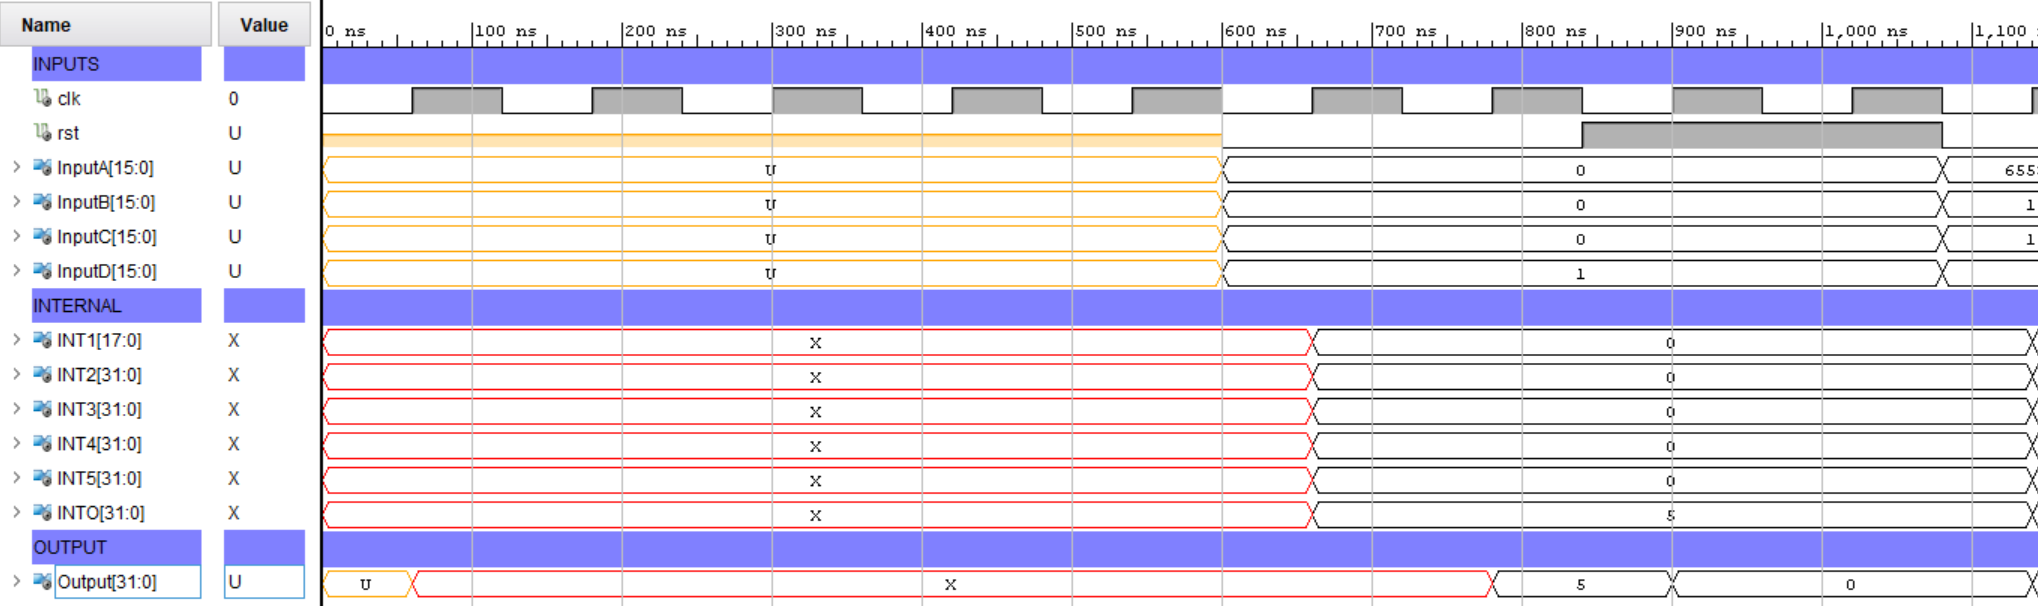
\includegraphics[width=\columnwidth]{Reports/Lab2/Waveforms/120ns_behavioural_global-reset.png}
\end{figure}
\subsection*{Waveform 2: Test Sequence}
\begin{figure}[H]
    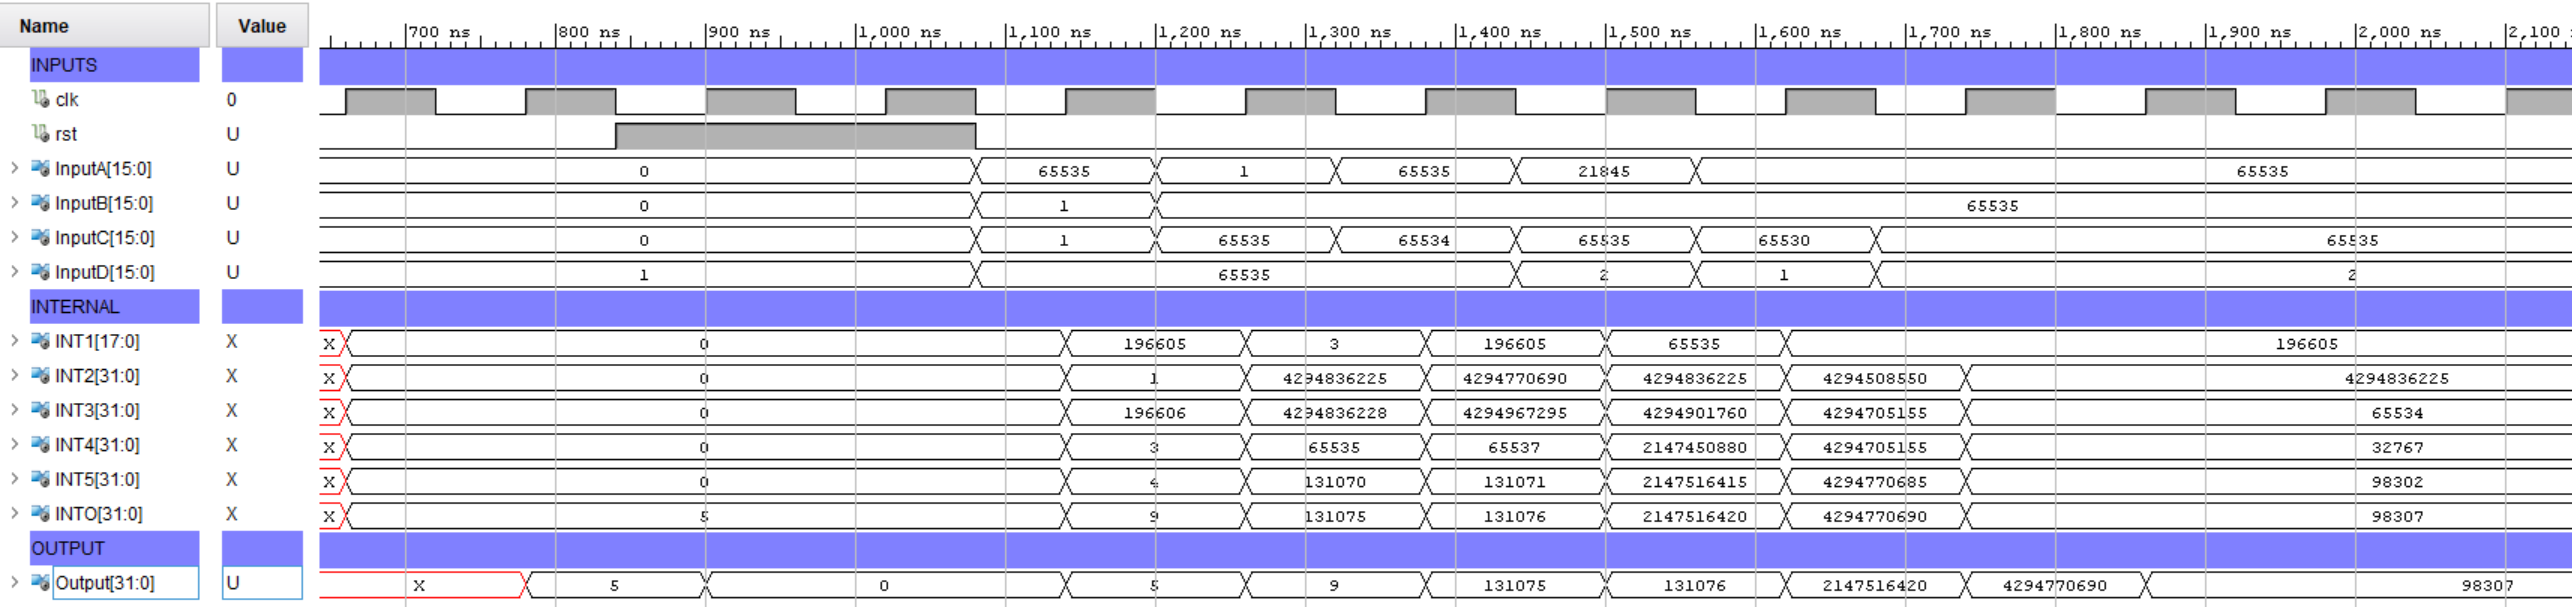
\includegraphics[width=\columnwidth]{Reports/Lab2/Waveforms/120ns_behavioural_test-sequence.png}
\end{figure}
\subsection*{Console Output}
\begin{figure}[H]
    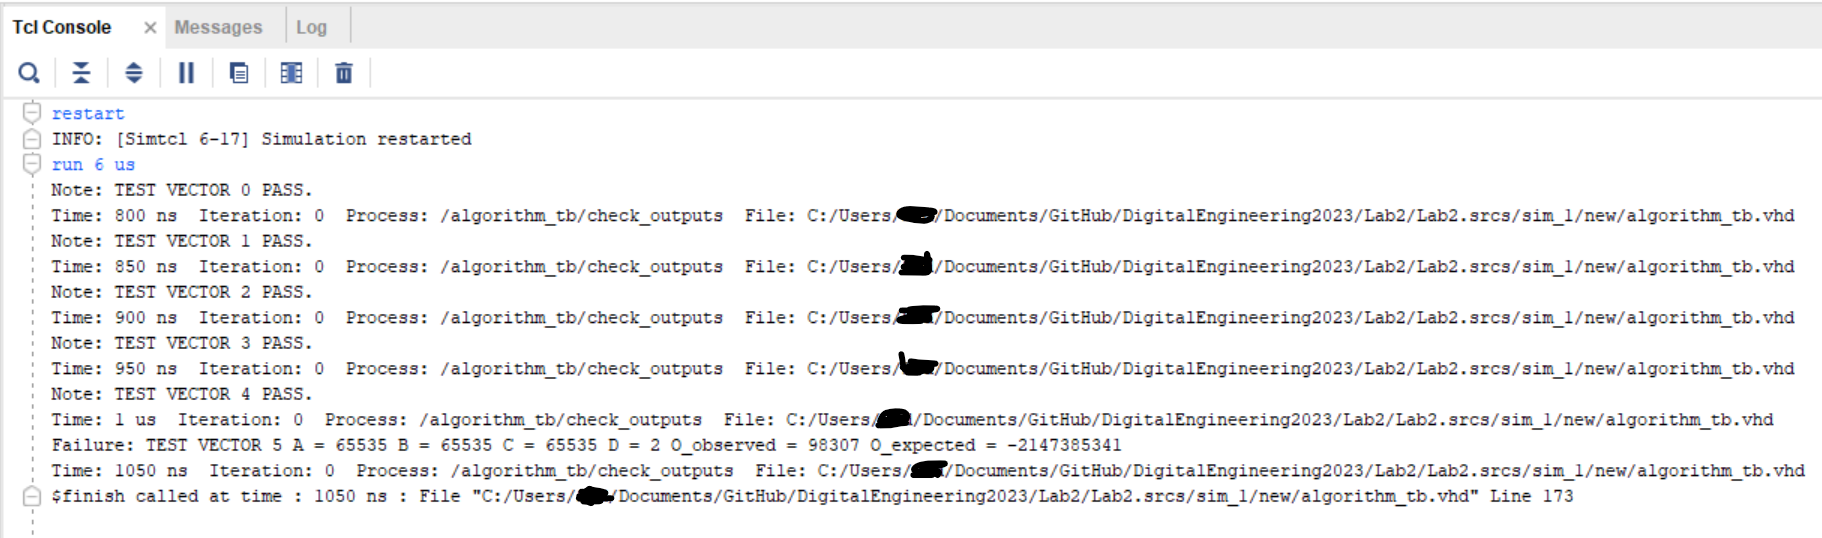
\includegraphics[width=\columnwidth]{Reports/Lab2/Waveforms/120ns_behavioural-console.png}
\end{figure}


\section*{1.1.3 Design Runs - WNS}
\begin{figure}[H]
    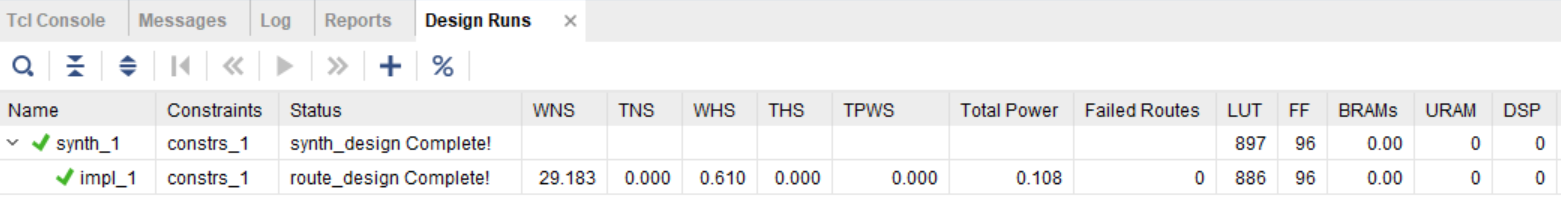
\includegraphics[width=\columnwidth]{Reports/Lab2/Waveforms/design_runs-WNS.png}
\end{figure}
The implementation process consists of 3 steps: `Translate', where the netlist and constraints are merged into an Xilinx design file. `Map', where the design is implemented on the target device. And finally, `place and route', where the components are placed and routes are designed according to the timing constraints. This process incorporates proprietary and classified algorithms that rely on random factors, therefore, the same design will never be implemented twice.

After the `place and route' step is complete, the tools will be able to provide an estimate of all the propagation delays for all signals within the entire device after the `static timing analysis' step. With the timing information, the tools can calculate the `worst negative slack' (WNS).

From the WNS value we got from our implementation, we can run our circuit with a clock signal as fast as 90.817ns, or around 11.01MHz.


\section*{1.1.4 Timing Simulation (120ns Clock)}
\subsection*{Waveform 1: Global Initialisation/Reset}
\begin{figure}[H]
    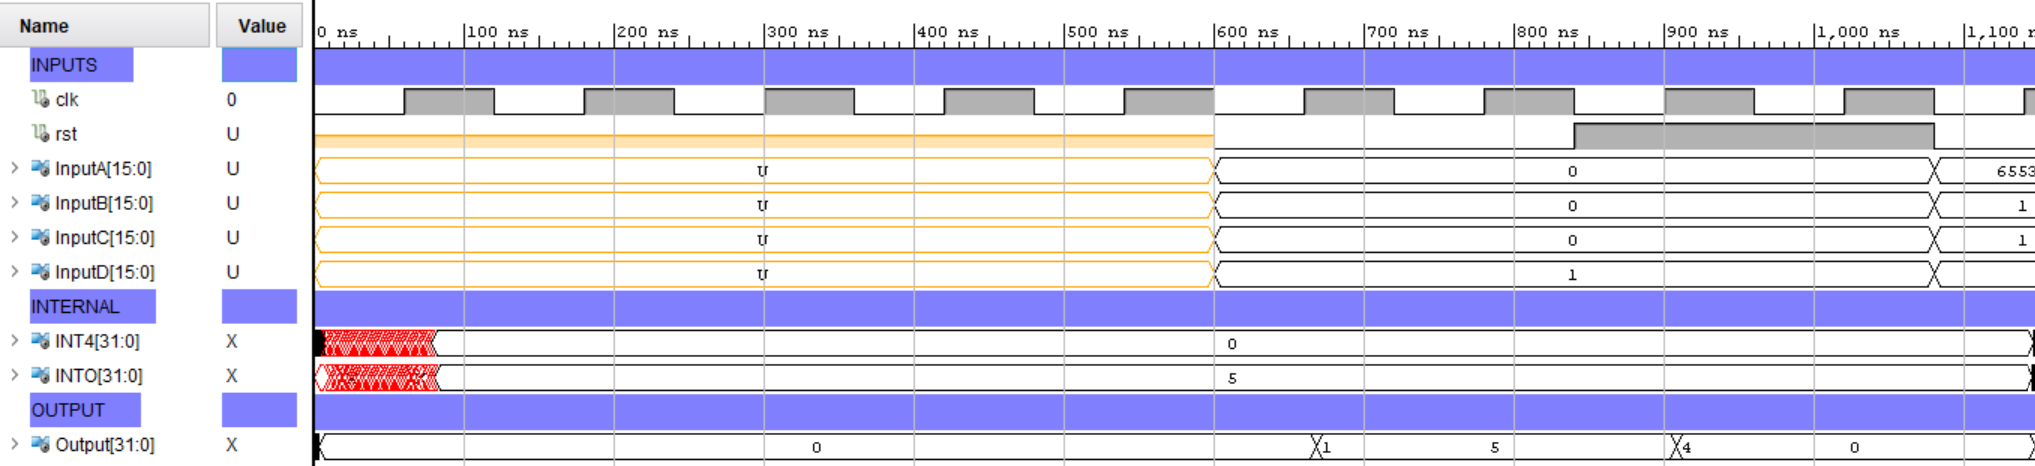
\includegraphics[width=\columnwidth]{Reports/Lab2/Waveforms/120ns_timing_sim-global-reset.png}
\end{figure}
\subsection*{Waveform 2: Test Sequence}
\begin{figure}[H]
    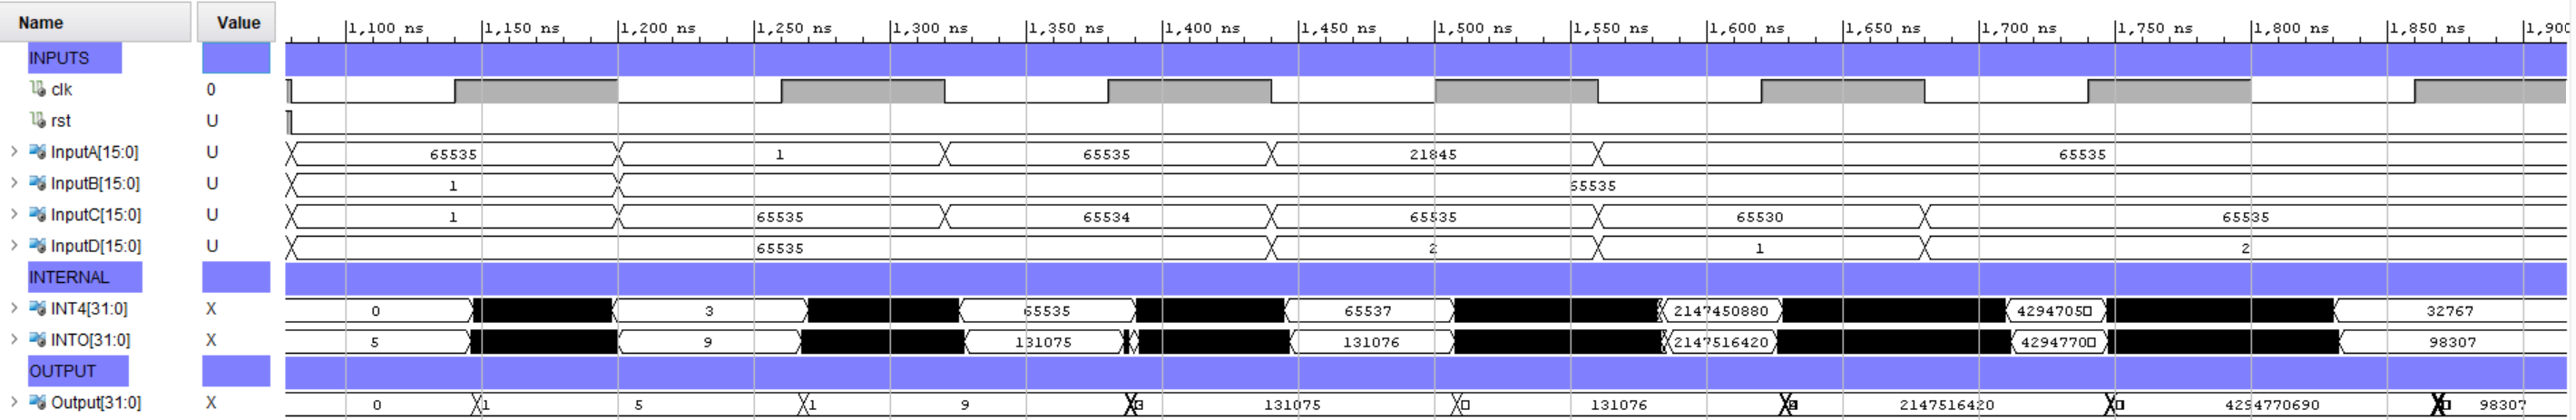
\includegraphics[width=\columnwidth]{Reports/Lab2/Waveforms/120ns_timing_sim-test-sequence.png}
\end{figure}
\subsection*{Console Output}
\begin{figure}[H]
    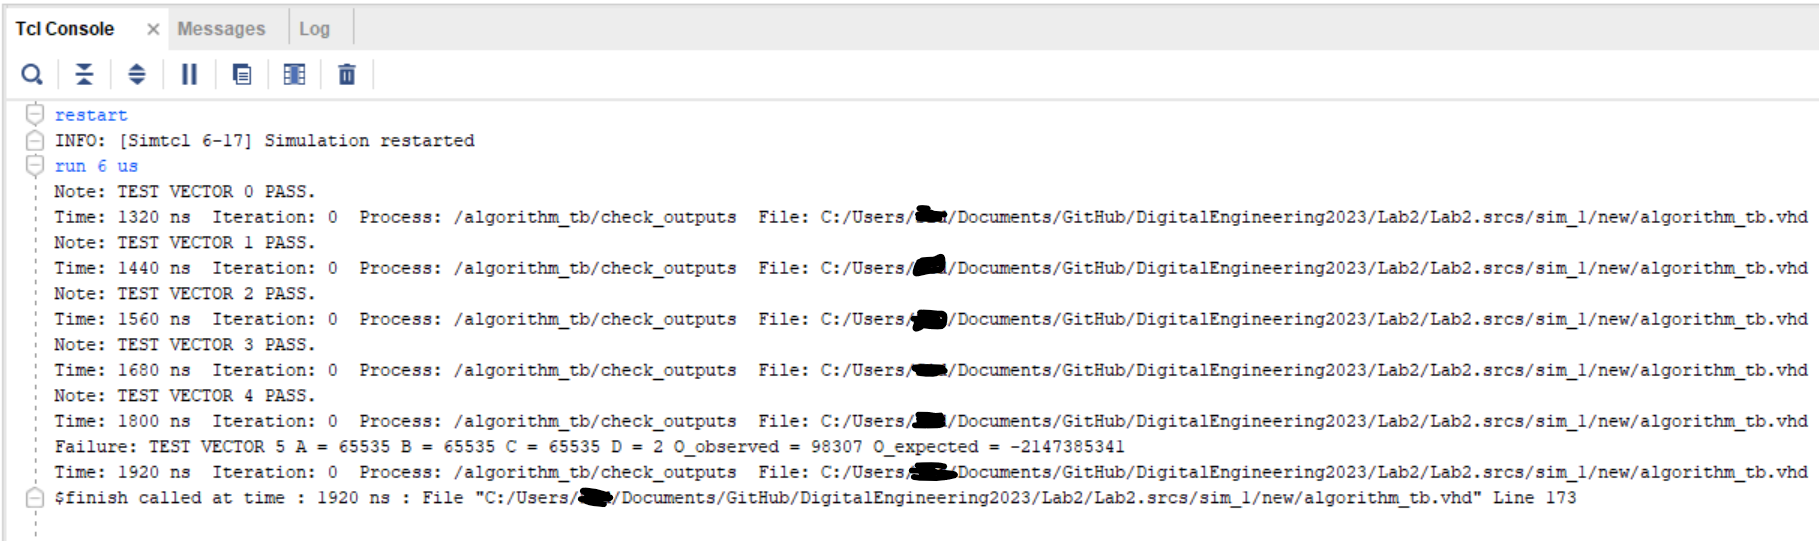
\includegraphics[width=\columnwidth]{Reports/Lab2/Waveforms/120ns_timing_sim-console.png}
\end{figure}


\section*{1.1.5 Timing Simulation (50ns Clock)}
\subsection*{Waveform 1: Global Initialisation/Reset}
\begin{figure}[H]
    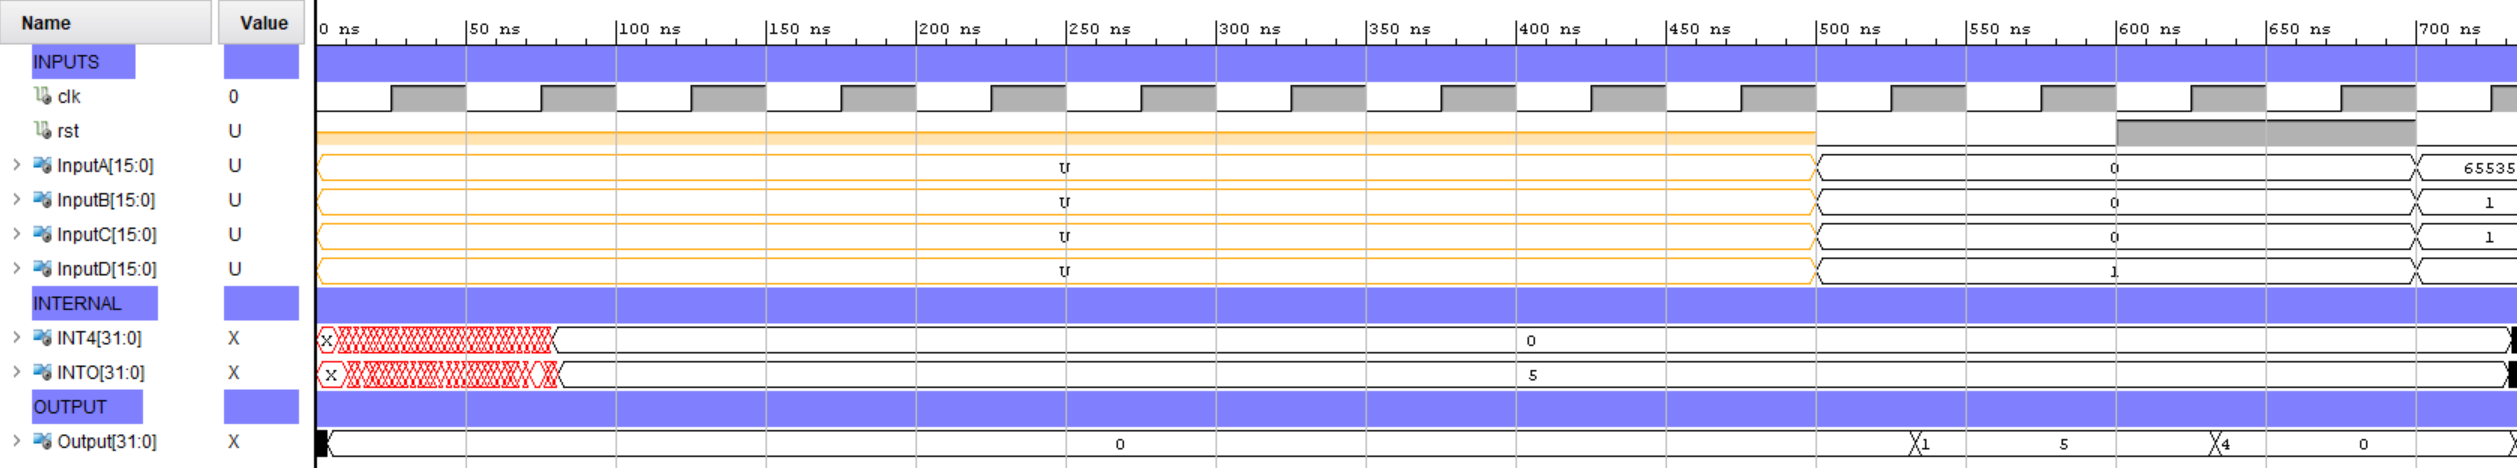
\includegraphics[width=\columnwidth]{Reports/Lab2/Waveforms/50ns_timing_sim-global-reset.png}
\end{figure}
\subsection*{Waveform 2: Test Sequence (Vector \#1-3)}
\begin{figure}[H]
    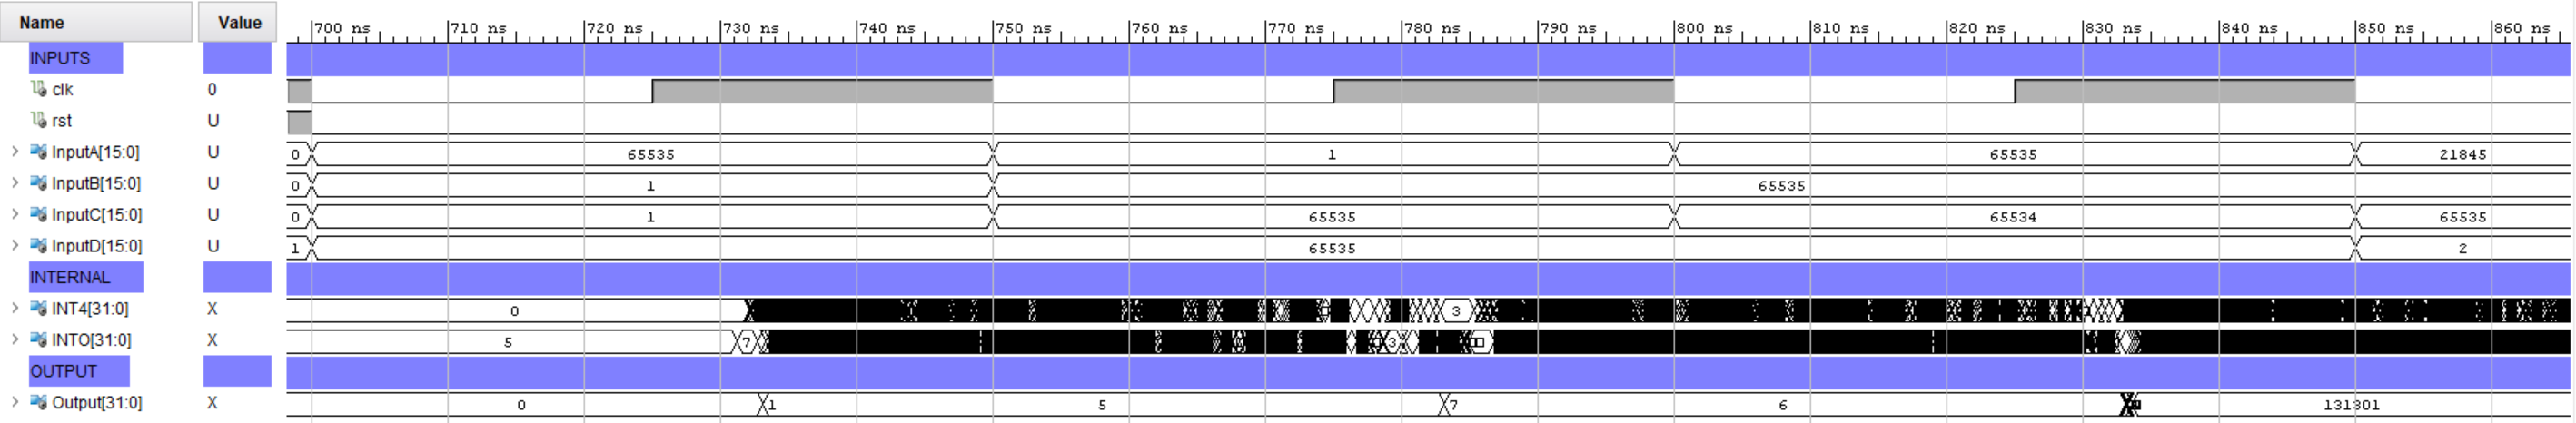
\includegraphics[width=\columnwidth]{Reports/Lab2/Waveforms/50ns_timing_sim-test-sequence-1-3.png}
\end{figure}
\subsection*{Waveform 3: Test Sequence (Vector \#3-6)}
\begin{figure}[H]
    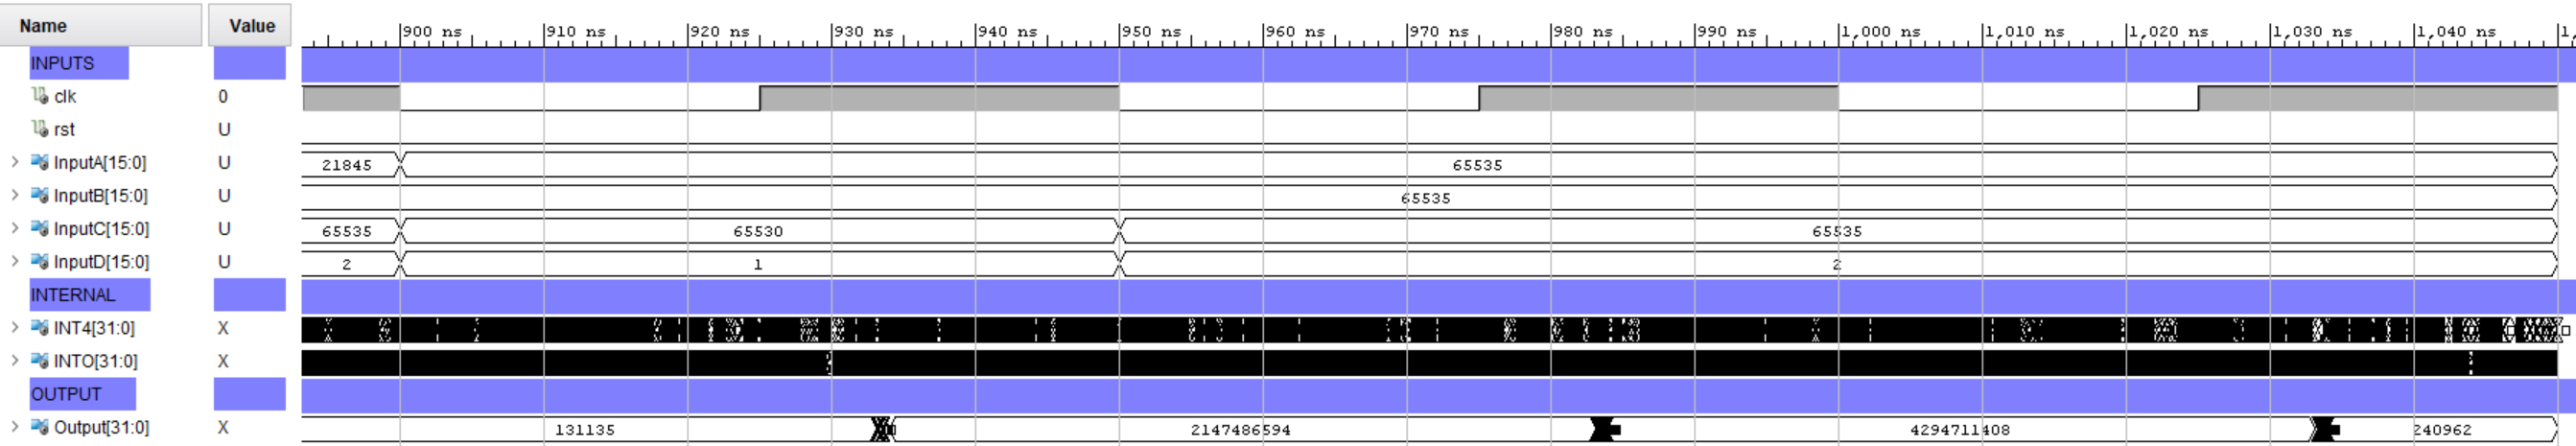
\includegraphics[width=\columnwidth]{Reports/Lab2/Waveforms/50ns_timing_sim-test-sequence-3-6.png}
\end{figure}
\subsection*{Console Output}
\begin{figure}[H]
    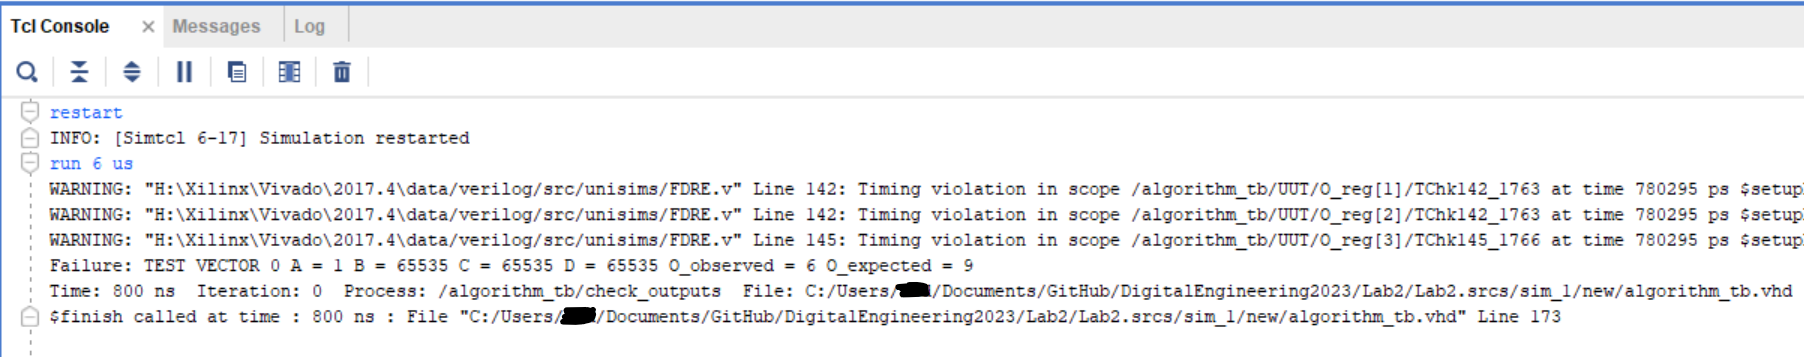
\includegraphics[width=\columnwidth]{Reports/Lab2/Waveforms/50ns_timing_sim-console.png}
\end{figure}


\section*{1.1.6 Analysis of Results}
\subsection*{Question 1}
During the synthesis stage to generate the netlist, the tools will process the project VHDL files to check syntax and optimise designs. Due to this optimisation step, the tools will optimise across all hierarchy levels (unless it's explicitly told not to do so), therefore, hierarchy is often destroyed. 

As the implementation stage needs to be run for the timing simulations, these simulations are based on the netlist. Therefore, we can only see the INT4 and INTO internal signals, all others have been destroyed by the tools for optimisation purposes.

\subsection*{Question 2}
As propagation delays aren't taken into account with a simple behavioural simulation, we can notice everything changes at the exact edge of the clock. The post-implementation timing simulation on the other hand takes into account of these delays, therefore, changes only happen once the signal has propagated and before that, intermediate transient values are produced due to unequal propagation.

Comparing the `INTO' signals, we see that the value changes to the correct one only after half a clock cycle of metastability, this is due to unequal propagation delays. The `Output` signal is slightly delays relative to the rising clock edge, and there seems to be an intermediate transient value, likely caused by the metastability of `INTO'.

\subsection*{Question 3}
In the simulation results from 1.1.4, we say `INTO' metastability lasting only around half a clock cycle, in the waveform from 1.1.5, we see metastability throughout INTO. We can also see the increase in metastability as the simulation progresses; in Waveform 2 (Vector \#1-3), there are a few moments where the value stays fixed for a nanosecond or two, but in Waveform 3 (Vector \#3-6), the output for INTO turns into a dark black rectangle.

The behaviour for the Output signal is also quite consistent with the one from 1.1.4, the only difference being the Output is incorrect (due to the metastable INTO). But we can notice as INTO metastability increases in Waveform 2, there seems to be an increase in metastable transient values between register outputs.


\chapter*{Task B: Tool Optimisations}

\section*{1.2.1 Design Runs With Varying Timing Contraints}
\subsection*{80ns Clock Period}
\begin{figure}[H]
    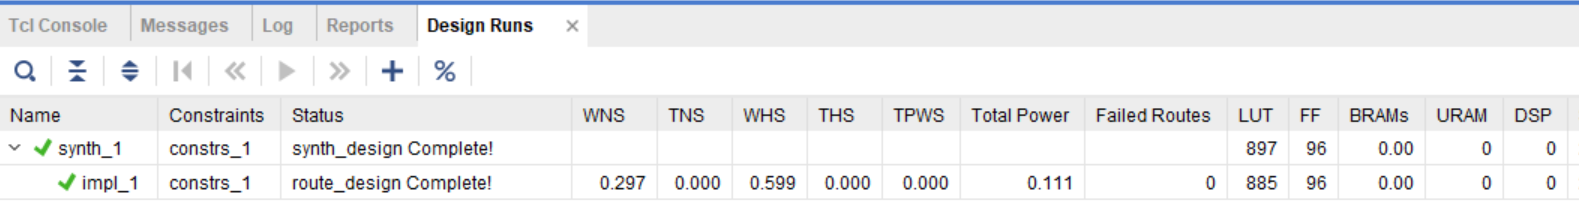
\includegraphics[width=\columnwidth]{Reports/Lab2/Waveforms/80ns_design-runs.png}
\end{figure}
From the WNS value we got from our implementation with an 80ns clock, we can run our circuit with a clock signal as fast as 79.703ns, or around 12.55MHz. With an 80ns clock signal in the testbench, we can indeed verify that the implementation works as the self-checking testbench passes.

\subsection*{75ns Clock Period}
\begin{figure}[H]
    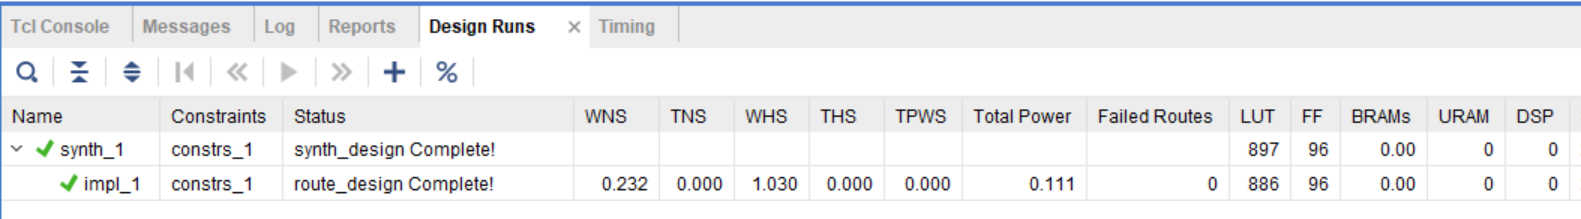
\includegraphics[width=\columnwidth]{Reports/Lab2/Waveforms/75ns_design-runs.png}
\end{figure}
From the WNS value we got from our implementation with a 75ns clock, we can run our circuit with a clock signal as fast as 74.268ns, or around 13.37MHz. Running the testbench with a 75ns simulated clock period, we can notice a fail in test vector \#4, where the inputs, A, B and C are 65535, and D is 2. Test vectors \#0-3 all pass. This can be explained as the WNS is only 0.232ns, this is such a small margin to work with and due to propagation delays and other limitations of a physical (real-life) device, this margin cannot be maintained.

\subsection*{70ns Clock Period}
\begin{figure}[H]
    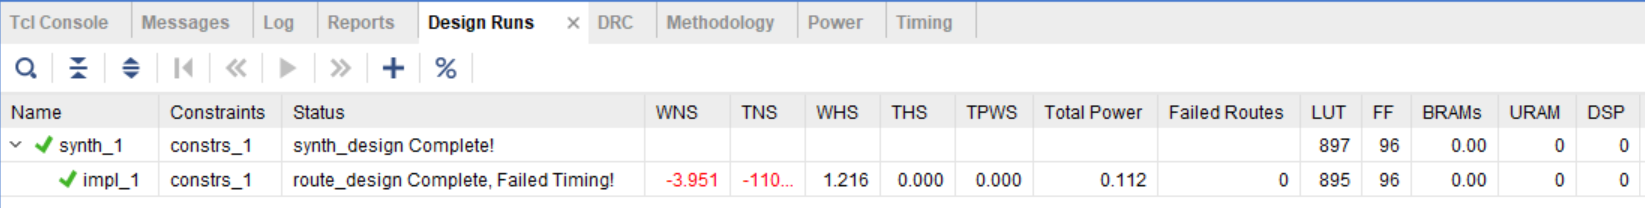
\includegraphics[width=\columnwidth]{Reports/Lab2/Waveforms/70ns_design-runs.png}
\end{figure}
This time, Xilinx couldn't meet the timing requirements that we set. With the displayed value, the maximum clock period has to be 73.951ns, or around 13.52MHz. It is however surprising that, just like for the 75ns clock period above, test vectors \#0-3 are passing, and only vector \#4 is failing instead of all of them.

\subsection*{Explanation}
As there are an infinite number of device arrangements for the logic, the process of implementation is an iterative one. The Xilinx tools will iterate until an implementation that complies with the defined timing constraints is found. After it has tried hard enough (iterated a maximum defined number of times), the tools may not be able to find a configuration that complies with the constraints, in this case, it will display a negative value in red, meaning that a valid clock period where the circuit will work is off by that value. Running a timing simulation when the timing is not met results in a lot of metastabilities within the internal signals, which leads to inaccurate and extremely unstable outputs and failing testbenches.

\section*{1.2.2 Setup Violation and Critical Path}
Setup time relates to the short duration required for a signal to be present before the clock edge for a sequential device. When this condition is not met, a setup violation will arise. To mitigate this violation, the clock period can be decreased, allowing for more time for the clock signal to propagate, or the delay of the incoming data path logic can be reduced. This will result in an increase in the critical path.

\section*{1.2.3 Post-Route Timing Report: Max Path Delay}
\begin{figure}[H]
    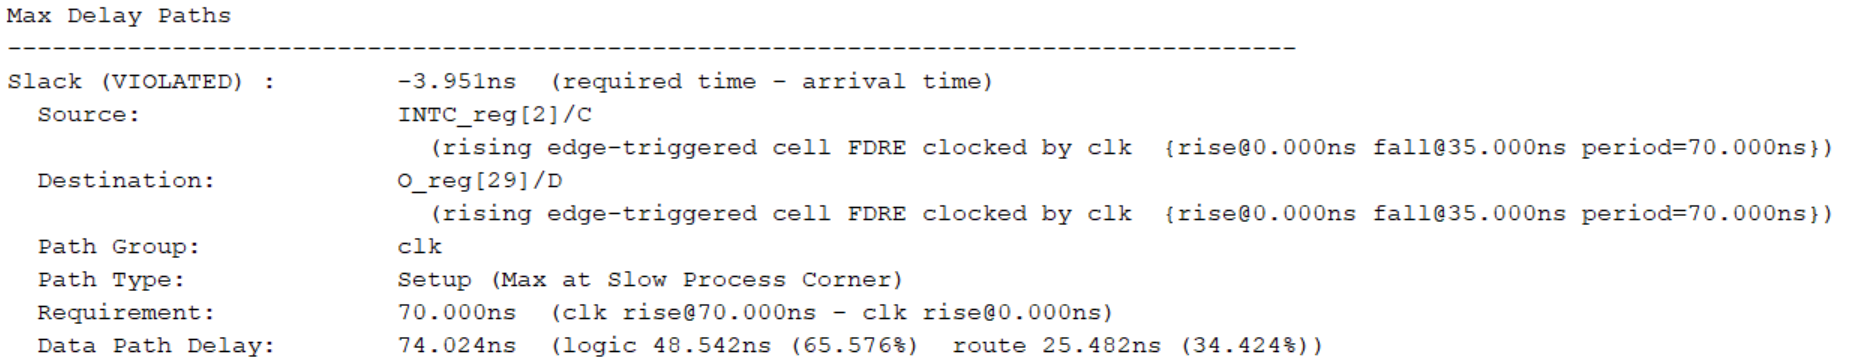
\includegraphics[width=\columnwidth]{Reports/Lab2/Waveforms/1.2.3_max-path-delay.png}
\end{figure}


\chapter*{Task C: Logic Optimisations}

\section*{1.3.1 Modified Algorithm Circuit}
\subsection*{Modified VHDL Code}
\inputminted[firstline=23]{vhdl}{"../../Lab2/Lab2.srcs/sources_1/imports/Digital Engineering/Algorithm.vhd"}

\subsection*{Design Runs}
\subsubsection*{70ns Clock Period}
\begin{figure}[H]
    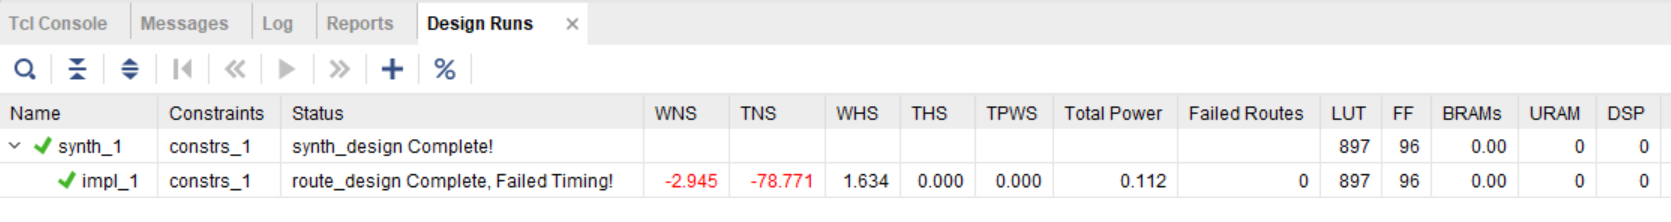
\includegraphics[width=\columnwidth]{Reports/Lab2/Waveforms/taskc_70ns_design-runs.png}
\end{figure}
Although this timing constraint still fails, we can see an improvement of almost 1ns when compared to the pre-modification case.

\subsubsection*{80ns Clock Period}
\begin{figure}[H]
    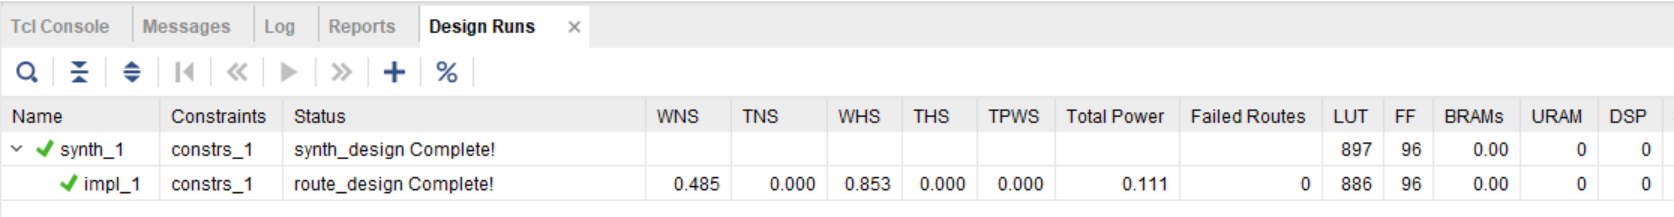
\includegraphics[width=\columnwidth]{Reports/Lab2/Waveforms/taskc_80ns_design-runs.png}
\end{figure}
In this case, the timing constraint passes. When compared to the pre-modification case, we can notice a drastic improvement of 189ns.

\end{document}
